% ======================================================================
%  PHỤ LỤC: BIÊN BẢN KIỂM THỬ HỆ THỐNG THEO VAI TRÒ
%  (sinh tự động từ bộ kiểm thử E2E Playwright chạy trên hệ thống thật)
% ======================================================================
\clearpage
\phantomsection
\addcontentsline{toc}{section}{Phụ lục. Biên bản kiểm thử hệ thống theo vai trò}
\markboth{Phụ lục — Kiểm thử}{Phụ lục — Kiểm thử}

\begin{center}\textbf{\large PHỤ LỤC. BIÊN BẢN KIỂM THỬ HỆ THỐNG THEO VAI TRÒ}\end{center}
\smallskip

Toàn bộ kịch bản kiểm thử dưới đây được \textbf{tự động hoá} bằng Playwright và thực thi \textbf{trực tiếp trên hệ thống đang chạy} (không dùng dữ liệu giả lập), bao trùm bốn luồng nghiệp vụ chính của TownHub. Điểm cốt lõi: kịch bản được xây dựng \textit{theo vai trò} — mỗi vai trò đăng nhập bằng tài khoản riêng và chỉ thực hiện đúng phần việc được phân quyền trong quy trình, thay vì để một tài khoản quản trị làm toàn bộ. Nhờ đó biên bản đồng thời kiểm chứng được cả nghiệp vụ (happy case) lẫn cơ chế kiểm soát truy cập/tách bạch nhiệm vụ (side case — kỳ vọng bị chặn \texttt{403}).

\textbf{Môi trường kiểm thử:}
\begin{itemize}[leftmargin=1.5em,itemsep=1pt,topsep=2pt]
  \item \textbf{Backend:} ASP.NET Core .NET 8, chạy tại \texttt{localhost:5267}; CSDL PostgreSQL (Neon).
  \item \textbf{Frontend:} Next.js 16 (React 19), chạy tại \texttt{localhost:3000}.
  \item \textbf{Dịch vụ OCR:} worker nền xử lý hàng đợi; ở môi trường kiểm thử dùng engine mô phỏng nên job OCR chạy đến trạng thái \texttt{COMPLETED} (mô hình OCR thực tế được đánh giá riêng ở Chương~2).
  \item \textbf{Công cụ:} Playwright (trình duyệt Chromium), chạy tuần tự một luồng để không quá tải CSDL đám mây.
  \item \textbf{Tài khoản:} 6 tài khoản ứng với 6 vai trò RBAC (Quản trị viên, Ban quản lý, Kỹ sư trưởng, Kỹ thuật viên, Kế toán, Cư dân).
\end{itemize}

\textbf{Kết quả tổng hợp:} \textbf{40/40} ca kiểm thử chức năng \textbf{ĐẠT} (20 ca thao tác hợp lệ + 20 ca kiểm soát/từ chối truy cập \texttt{403}), kèm 19 lượt chụp màn hình minh hoạ giao diện theo vai trò. Chi tiết ở các bảng và hình bên dưới.

\medskip
\textbf{Bảng PL.1. Tổng hợp kết quả theo nhóm chức năng}

\begin{center}{\small\renewcommand{\arraystretch}{1.2}
\begin{tabular}{|>{\raggedright\arraybackslash}p{0.40\linewidth}|c|c|c|}
\hline
\rowcolor{gray!15}\textbf{Nhóm chức năng} & \textbf{Happy} & \textbf{Side} & \textbf{Đạt} \\ \hline
Xác thực \& Phân quyền (Auth/RBAC) & 6 & 5 & 11/11 \\ \hline
Luồng Sự cố (Cư dân → BQL → KTV) & 3 & 4 & 7/7 \\ \hline
Luồng Mua sắm \& OCR (KST → BQL → Kế toán) & 4 & 4 & 8/8 \\ \hline
Luồng Tài sản (KST tạo · Kế toán vận hành) & 4 & 4 & 8/8 \\ \hline
Luồng Bảo trì / Work Order (BQL giao · KTV thực thi) & 3 & 3 & 6/6 \\ \hline
\rowcolor{gray!15}\textbf{Tổng} & \textbf{20} & \textbf{20} & \textbf{40/40} \\ \hline
\end{tabular}}\end{center}

\medskip
\textbf{Bảng PL.2. Ma trận phân quyền theo vai trò (kiểm chứng bằng kiểm thử)}

\noindent Ký hiệu: \checkmark{} = được phép (kiểm thử happy \texttt{200}); $\times$ = bị chặn (kiểm thử side \texttt{403}). Viết tắt vai trò: QTV = Quản trị viên, BQL = Ban quản lý, KST = Kỹ sư trưởng, KTV = Kỹ thuật viên, KT = Kế toán, CD = Cư dân.

\begin{center}{\small\renewcommand{\arraystretch}{1.25}
\begin{tabular}{|>{\raggedright\arraybackslash}p{0.34\linewidth}|c|c|c|c|c|c|}
\hline
\rowcolor{gray!15}\textbf{Hành động nghiệp vụ} & \textbf{QTV} & \textbf{BQL} & \textbf{KST} & \textbf{KTV} & \textbf{KT} & \textbf{CD} \\ \hline
Đăng nhập hệ thống & \checkmark & \checkmark & \checkmark & \checkmark & \checkmark & \checkmark \\ \hline
Xem danh sách tài sản & \checkmark & \checkmark & \checkmark & \checkmark & \checkmark & $\times$ \\ \hline
Tạo mới tài sản & \checkmark & $\times$ & \checkmark & $\times$ & $\times$ & $\times$ \\ \hline
Cập nhật / khấu hao tài sản & \checkmark & \checkmark & \checkmark & $\times$ & \checkmark & $\times$ \\ \hline
Tạo ticket sự cố & \checkmark & $\times$ & \checkmark & $\times$ & $\times$ & \checkmark \\ \hline
Phân công ticket cho KTV & \checkmark & \checkmark & \checkmark & $\times$ & $\times$ & $\times$ \\ \hline
Xử lý (chuyển trạng thái) ticket & \checkmark & $\times$ & \checkmark & \checkmark & $\times$ & $\times$ \\ \hline
Tạo phiếu yêu cầu mua sắm (PR) & \checkmark & \checkmark & \checkmark & $\times$ & $\times$ & $\times$ \\ \hline
Duyệt phiếu yêu cầu mua sắm & \checkmark & \checkmark & $\times$ & $\times$ & $\times$ & $\times$ \\ \hline
Xử lý OCR hoá đơn & \checkmark & $\times$ & $\times$ & $\times$ & \checkmark & $\times$ \\ \hline
Tạo lệnh công việc (Work Order) & \checkmark & \checkmark & \checkmark & $\times$ & $\times$ & $\times$ \\ \hline
Thực thi Work Order (đính minh chứng) & \checkmark & $\times$ & \checkmark & \checkmark & $\times$ & $\times$ \\ \hline
\end{tabular}}\end{center}

\smallskip
\noindent\textit{Nhận xét: ma trận thể hiện rõ nguyên tắc tách bạch nhiệm vụ — người đề xuất mua sắm (Kỹ sư trưởng) không được tự duyệt; Ban quản lý điều phối/giao việc nhưng không trực tiếp thực thi kỹ thuật; Kế toán phụ trách hoá đơn nhưng không được duyệt phiếu yêu cầu; Cư dân chỉ báo sự cố và tra cứu.}

% --------------------------------------------------------------
%  BẢNG CHI TIẾT TEST CASE (trang ngang)
% --------------------------------------------------------------
\begin{landscape}{\footnotesize\singlespacing\renewcommand{\arraystretch}{1.25}\setlength{\LTleft}{0pt}\setlength{\LTright}{0pt}
\textbf{Bảng PL.3. Chi tiết ca kiểm thử theo vai trò và kết quả thực tế}\par\smallskip
\begin{longtable}{|>{\raggedright\arraybackslash}p{0.07\linewidth}|>{\raggedright\arraybackslash}p{0.11\linewidth}|>{\raggedright\arraybackslash}p{0.30\linewidth}|>{\raggedright\arraybackslash}p{0.27\linewidth}|>{\raggedright\arraybackslash}p{0.13\linewidth}|c|}
\hline
\rowcolor{gray!20}\textbf{Mã} & \textbf{Vai trò} & \textbf{Kịch bản / thao tác} & \textbf{Kết quả mong đợi} & \textbf{Thực tế} & \textbf{KQ} \\ \hline
\endhead

\multicolumn{6}{|l|}{\cellcolor{blue!8}\textbf{A. Xác thực \& Phân quyền (Auth/RBAC)}} \\ \hline
TC-AUTH-01 & (mọi) & Đăng nhập với thông tin hợp lệ trên giao diện & Vào được dashboard, hiện menu theo quyền & Vào dashboard & \checkmark \\ \hline
TC-AUTH-03 & (mọi) & Đăng nhập sai mật khẩu & Báo lỗi, ở lại trang đăng nhập & Báo lỗi & \checkmark \\ \hline
TC-AUTH-04 & (mọi) & Bỏ trống tài khoản/mật khẩu & Chặn phía client, nhắc nhập & Bị chặn & \checkmark \\ \hline
TC-AUTH-05 & (mọi) & Đăng nhập qua API & Trả token JWT kèm danh sách quyền & Có token+quyền & \checkmark \\ \hline
TC-AUTH-06 & (mọi) & Đăng nhập API sai mật khẩu & Không trả token & Không token & \checkmark \\ \hline
TC-AUTH-07 & — & Gọi API bảo vệ khi chưa đăng nhập & Bị từ chối \texttt{401 Unauthorized} & \texttt{401} & \checkmark \\ \hline
TC-RBAC-a & Ban quản lý & Quyền trong JWT đúng thiết kế (có duyệt PR/phân công; không tạo ticket, không thực thi WO) & Khớp ma trận PL.2 & Khớp & \checkmark \\ \hline
TC-RBAC-b & Kỹ sư trưởng & Có tạo tài sản/ticket/WO, đề xuất PR; không duyệt PR, không OCR & Khớp ma trận PL.2 & Khớp & \checkmark \\ \hline
TC-RBAC-c & Kỹ thuật viên & Có xem tài sản, xử lý ticket, thực thi WO; không tạo ticket/WO/tài sản & Khớp ma trận PL.2 & Khớp & \checkmark \\ \hline
TC-RBAC-d & Kế toán & Có OCR/hoá đơn, cập nhật tài sản, báo cáo; không tạo tài sản, không duyệt PR & Khớp ma trận PL.2 & Khớp & \checkmark \\ \hline
TC-RBAC-e & Cư dân & Chỉ có tạo/xem ticket, xem thông báo; không xem tài sản, không duyệt & Khớp ma trận PL.2 & Khớp & \checkmark \\ \hline

\multicolumn{6}{|l|}{\cellcolor{blue!8}\textbf{B. Luồng Sự cố: Cư dân → Ban quản lý → Kỹ thuật viên}} \\ \hline
TC-INC-10 & Cư dân & Tạo ticket báo sự cố (mất điện hành lang) & Tạo thành công, sinh mã \texttt{TK-*} & Mã \texttt{TK-*} & \checkmark \\ \hline
TC-INC-11 & Cư dân & Thử xem danh sách tài sản & Bị chặn \texttt{403} & \texttt{403} & \checkmark \\ \hline
TC-INC-12 & Kỹ thuật viên & Thử tạo ticket & Bị chặn \texttt{403} (KTV không có quyền tạo) & \texttt{403} & \checkmark \\ \hline
TC-INC-13 & Ban quản lý & Phân công KTV xử lý ticket & Phân công thành công \texttt{200} & \texttt{200} & \checkmark \\ \hline
TC-INC-14 & Ban quản lý & Thử tự chuyển trạng thái (resolve) ticket & Bị chặn \texttt{403} (không có quyền xử lý) & \texttt{403} & \checkmark \\ \hline
TC-INC-15 & Kỹ thuật viên & Chuyển ticket sang trạng thái đang xử lý & Cập nhật thành công \texttt{200} & \texttt{200} & \checkmark \\ \hline
TC-INC-16 & Cư dân & Thử phân công ticket & Bị chặn \texttt{403} & \texttt{403} & \checkmark \\ \hline

\multicolumn{6}{|l|}{\cellcolor{blue!8}\textbf{C. Luồng Mua sắm \& OCR: Kỹ sư trưởng → Ban quản lý → Kế toán}} \\ \hline
TC-PRO-10 & Kỹ sư trưởng & Tạo và gửi duyệt phiếu yêu cầu (PR) & Tạo được, sinh mã \texttt{PR-*}, gửi duyệt & Mã \texttt{PR-*} & \checkmark \\ \hline
TC-PRO-11 & Kỹ sư trưởng & Thử tự duyệt PR do mình đề xuất & Bị chặn \texttt{403} (tách bạch nhiệm vụ) & \texttt{403} & \checkmark \\ \hline
TC-PRO-12 & Ban quản lý & Duyệt PR do Kỹ sư trưởng gửi & Duyệt thành công \texttt{200} & \texttt{200} & \checkmark \\ \hline
TC-PRO-13 & Kế toán & Thử duyệt PR & Bị chặn \texttt{403} & \texttt{403} & \checkmark \\ \hline
TC-PRO-14 & Cư dân & Thử tạo PR & Bị chặn \texttt{403} & \texttt{403} & \checkmark \\ \hline
TC-OCR-15 & Kế toán & Gửi hoá đơn cho OCR & Job được xử lý đến trạng thái kết thúc & \texttt{COMPLETED} & \checkmark \\ \hline
TC-OCR-16 & Ban quản lý & Thử gửi OCR hoá đơn & Bị chặn \texttt{403} (không có quyền hoá đơn) & \texttt{403} & \checkmark \\ \hline
TC-PRO-x & (kết hợp) & Chuỗi PR: đề xuất → gửi → duyệt hoàn tất & Vòng đời PR chạy đúng qua 2 vai trò & Đúng & \checkmark \\ \hline

\multicolumn{6}{|l|}{\cellcolor{blue!8}\textbf{D. Luồng Quản lý tài sản: Kỹ sư trưởng tạo · Kế toán vận hành}} \\ \hline
TC-AST-10 & Kỹ sư trưởng & Tạo mới tài sản (kèm nguyên giá, khấu hao) & Tạo thành công \texttt{200} & \texttt{200} & \checkmark \\ \hline
TC-AST-11 & Kỹ thuật viên & Thử tạo tài sản & Bị chặn \texttt{403} & \texttt{403} & \checkmark \\ \hline
TC-AST-12 & Kế toán & Thử tạo tài sản & Bị chặn \texttt{403} (chỉ được cập nhật) & \texttt{403} & \checkmark \\ \hline
TC-AST-13 & Kế toán & Xem tài sản + báo cáo bảng cân đối thử & Truy cập thành công \texttt{200} & \texttt{200} & \checkmark \\ \hline
TC-AST-14 & Kế toán & Cập nhật tài sản (kiểm tra phân quyền) & Được phép (không bị \texttt{403}) & Không \texttt{403} & \checkmark \\ \hline
TC-AST-15 & Kỹ thuật viên & Thử cập nhật tài sản & Bị chặn \texttt{403} & \texttt{403} & \checkmark \\ \hline
TC-AST-16 & Kỹ thuật viên & Xem danh sách tài sản & Truy cập thành công \texttt{200} & \texttt{200} & \checkmark \\ \hline
TC-AST-17 & Cư dân & Thử xem danh sách tài sản & Bị chặn \texttt{403} & \texttt{403} & \checkmark \\ \hline

\multicolumn{6}{|l|}{\cellcolor{blue!8}\textbf{E. Luồng Bảo trì / Work Order: Ban quản lý giao · Kỹ thuật viên thực thi}} \\ \hline
TC-WO-10 & Ban quản lý & Tạo lệnh công việc (Work Order) & Tạo được, sinh mã \texttt{WO-*} & Mã \texttt{WO} & \checkmark \\ \hline
TC-WO-11 & Ban quản lý & Phân công KTV cho Work Order & Phân công thành công \texttt{200} & \texttt{200} & \checkmark \\ \hline
TC-WO-12 & Ban quản lý & Thử tự thực thi WO (đính minh chứng) & Bị chặn \texttt{403} (chỉ giao, không thực thi) & \texttt{403} & \checkmark \\ \hline
TC-WO-13 & Kỹ thuật viên & Thử tạo Work Order & Bị chặn \texttt{403} & \texttt{403} & \checkmark \\ \hline
TC-WO-14 & Kỹ thuật viên & Thực thi WO: đính kèm ảnh minh chứng & Thực thi thành công \texttt{200} & \texttt{200} & \checkmark \\ \hline
TC-WO-15 & Kế toán & Thử xem danh sách Work Order & Bị chặn \texttt{403} & \texttt{403} & \checkmark \\ \hline
\end{longtable}}\end{landscape}

% --------------------------------------------------------------
%  ẢNH MINH HOẠ
% --------------------------------------------------------------
\clearpage
\textbf{Ảnh minh hoạ 1 — Dashboard hiển thị theo vai trò (menu chức năng thay đổi theo quyền).}

\begin{figure}[H]\centering
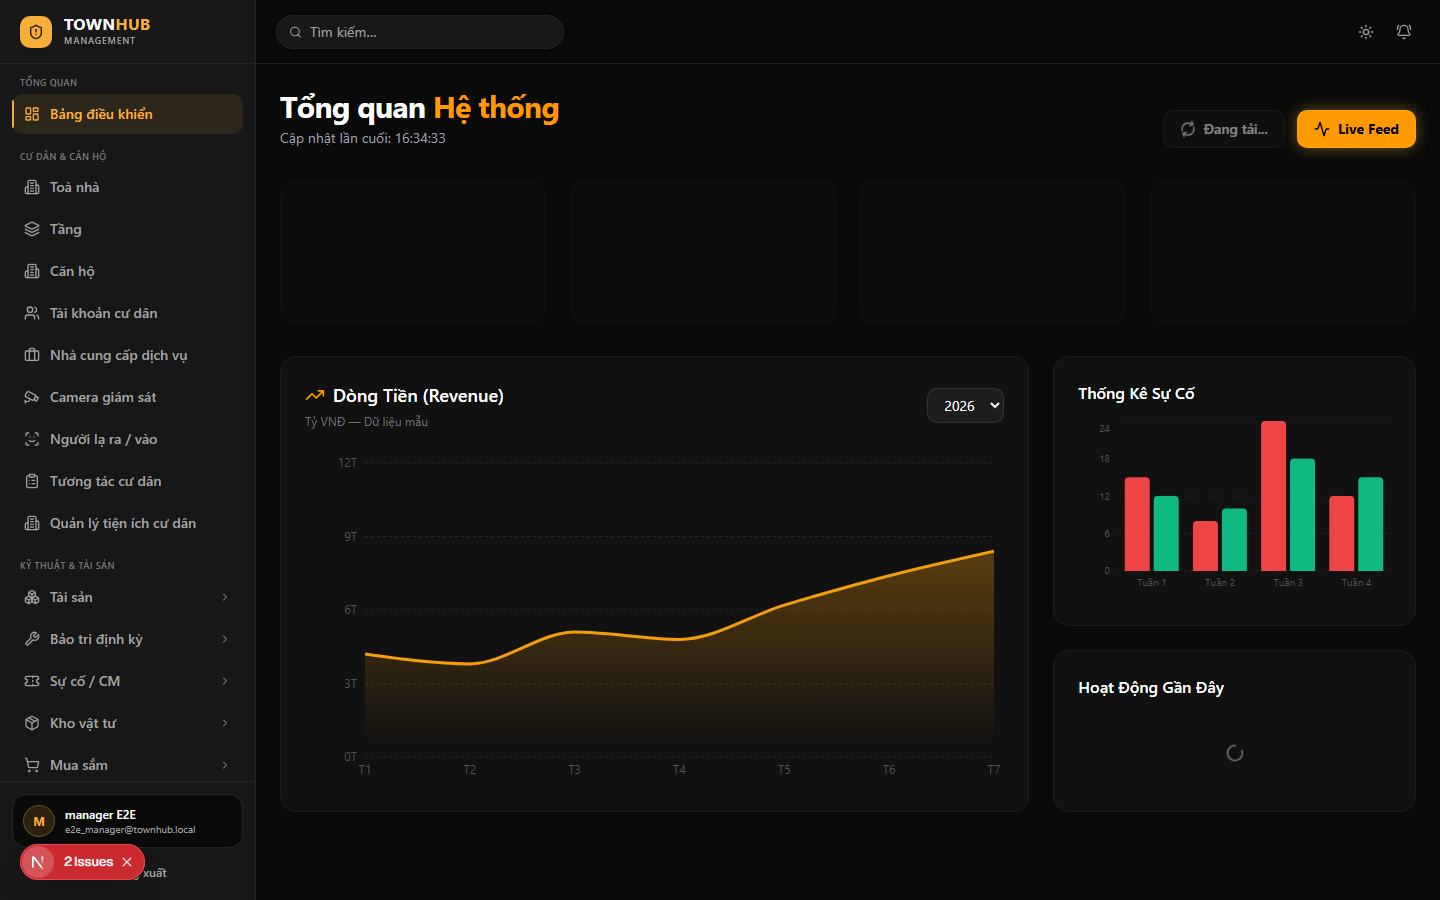
\includegraphics[width=\linewidth,height=0.44\textheight,keepaspectratio]{images/tc_role_manager_dashboard.png}
\caption*{\small Hình PL.1. Giao diện đăng nhập vai trò \textbf{Ban quản lý}.}
\end{figure}
\begin{figure}[H]\centering
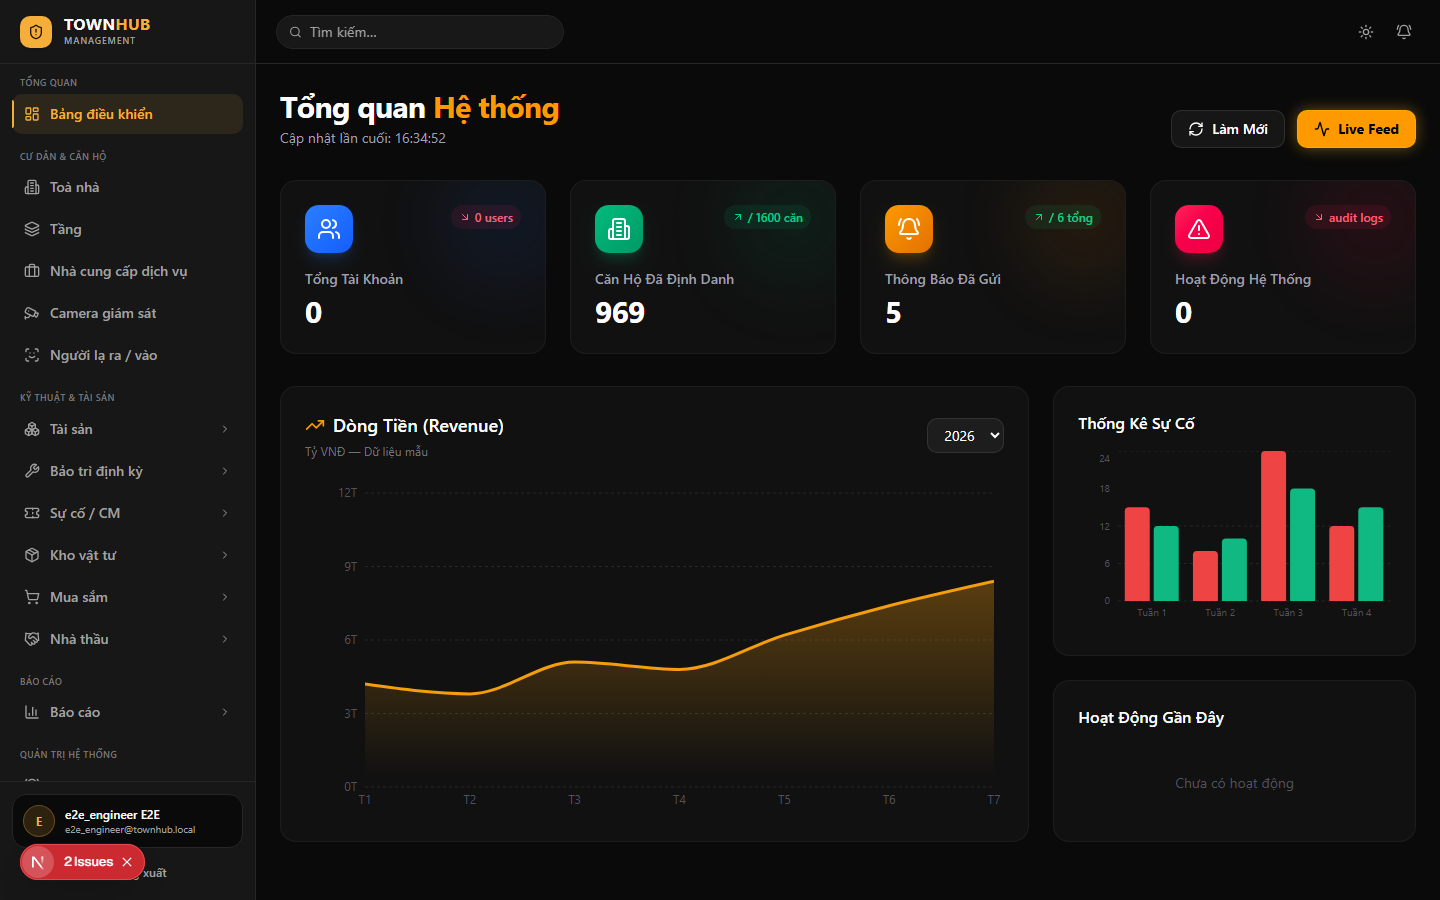
\includegraphics[width=\linewidth,height=0.44\textheight,keepaspectratio]{images/tc_role_engineer_dashboard.png}
\caption*{\small Hình PL.2. Giao diện đăng nhập vai trò \textbf{Kỹ sư trưởng}.}
\end{figure}
\begin{figure}[H]\centering
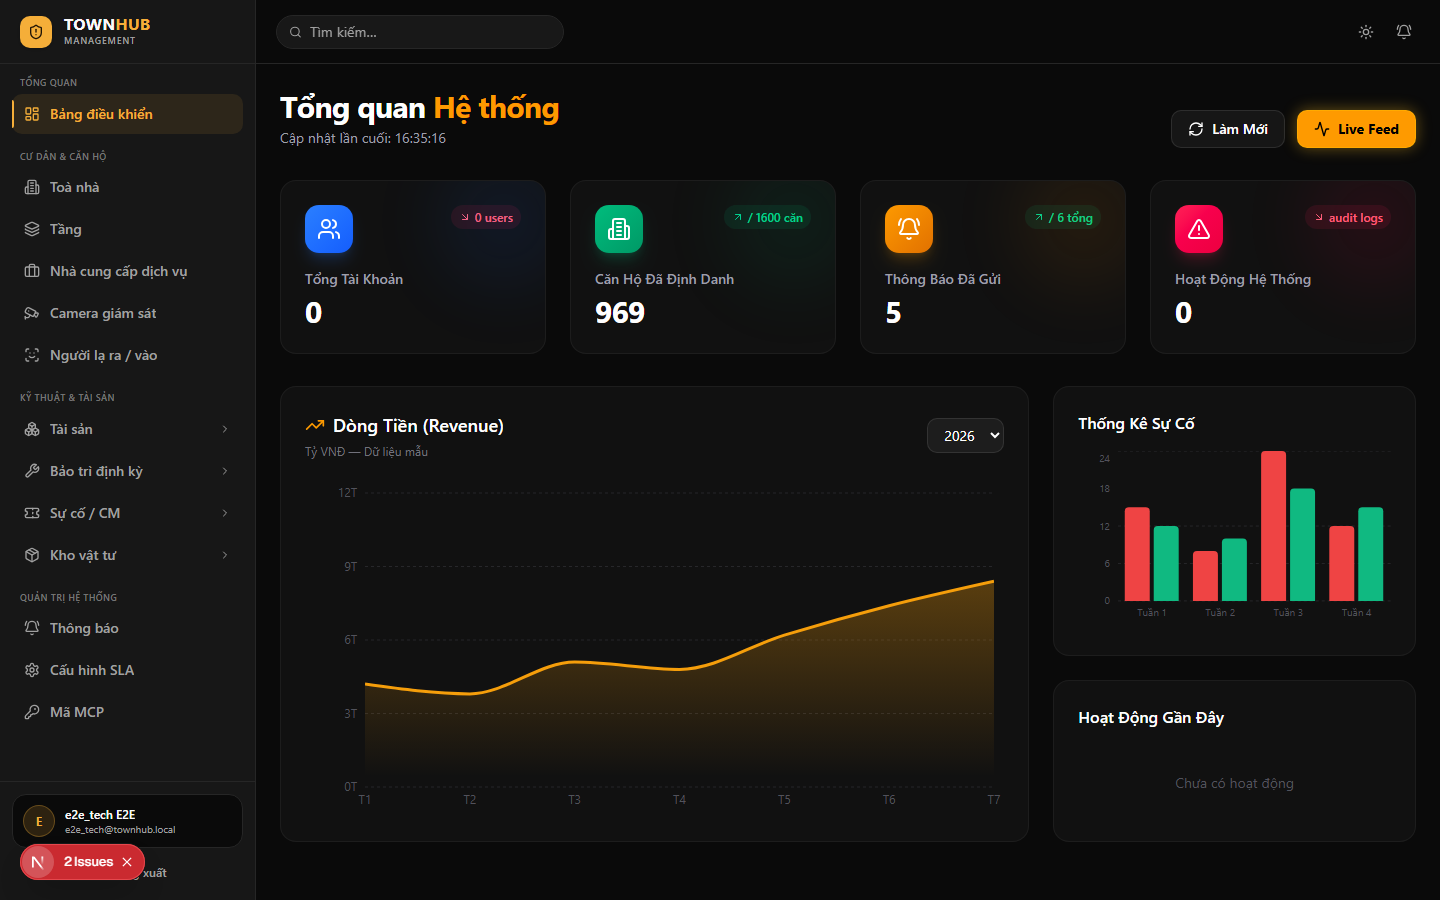
\includegraphics[width=\linewidth,height=0.44\textheight,keepaspectratio]{images/tc_role_technician_dashboard.png}
\caption*{\small Hình PL.3. Giao diện đăng nhập vai trò \textbf{Kỹ thuật viên}.}
\end{figure}
\clearpage
\begin{figure}[H]\centering
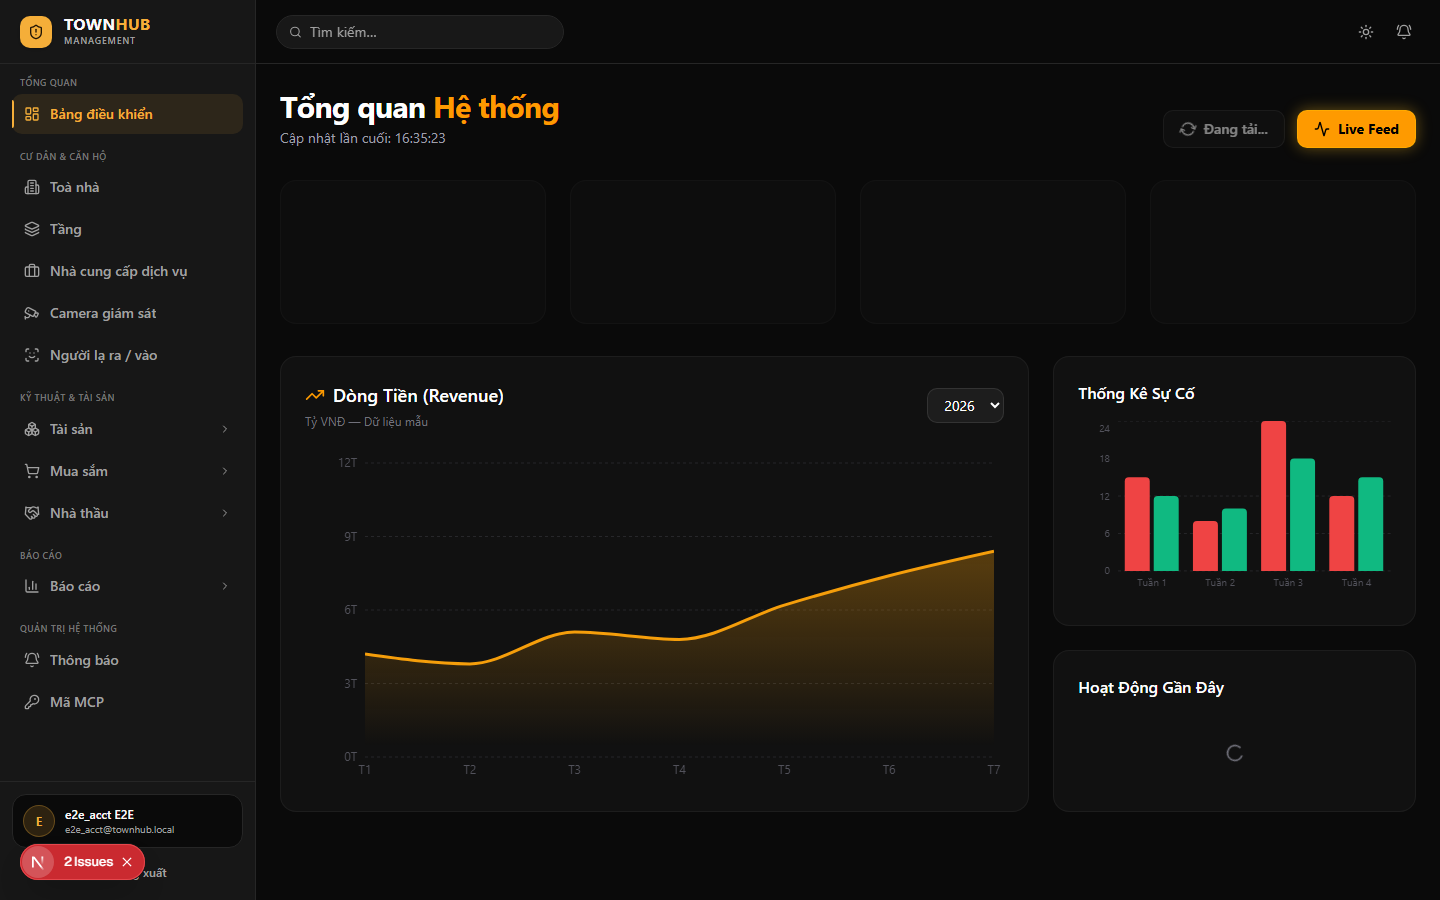
\includegraphics[width=\linewidth,height=0.44\textheight,keepaspectratio]{images/tc_role_accountant_dashboard.png}
\caption*{\small Hình PL.4. Giao diện đăng nhập vai trò \textbf{Kế toán}.}
\end{figure}
\begin{figure}[H]\centering
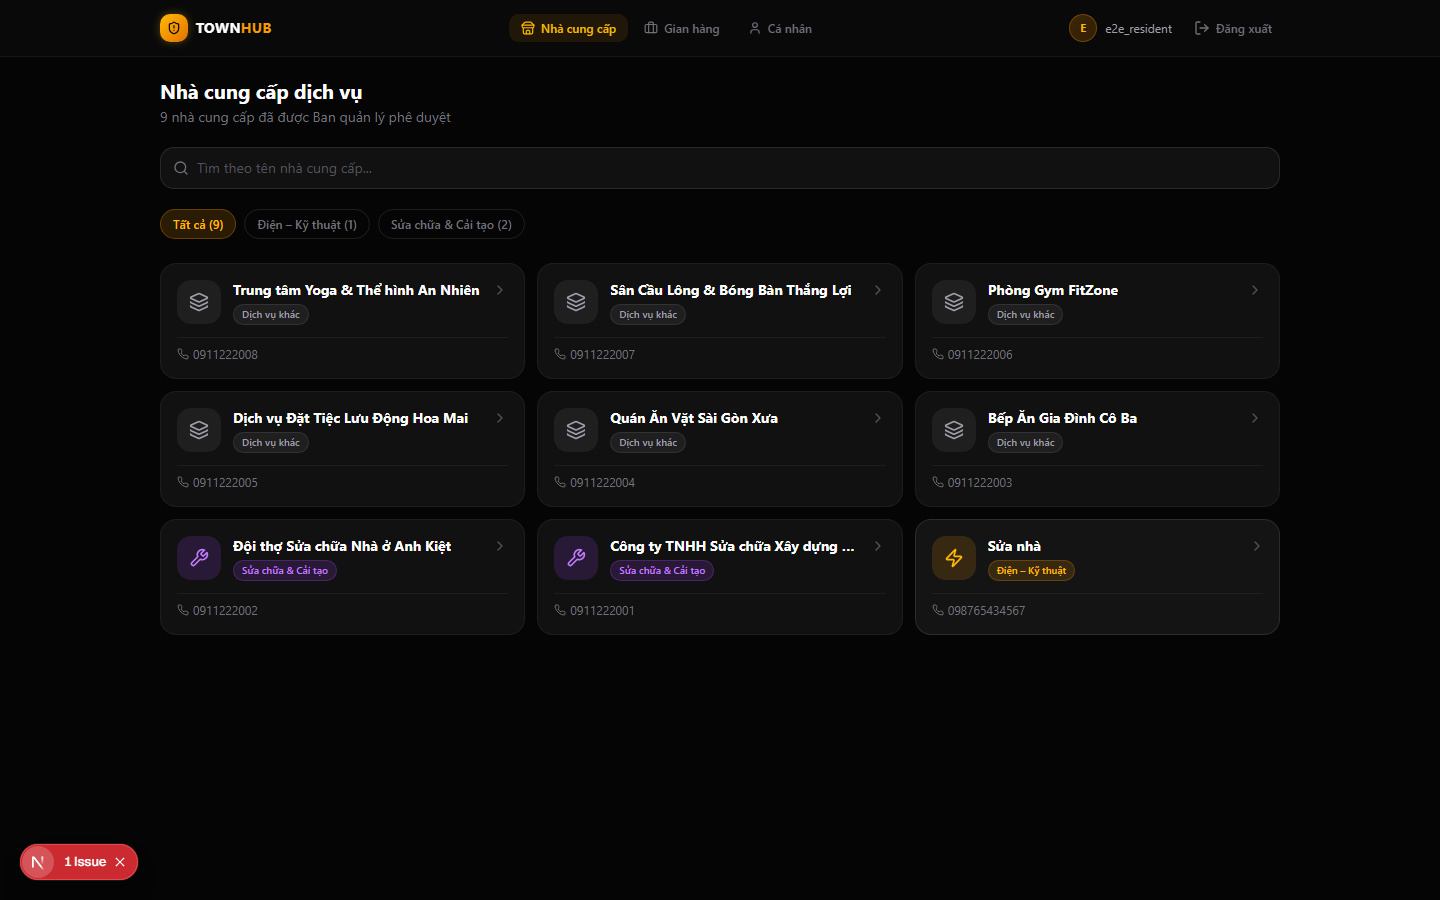
\includegraphics[width=\linewidth,height=0.44\textheight,keepaspectratio]{images/tc_role_resident_dashboard.png}
\caption*{\small Hình PL.5. Giao diện đăng nhập vai trò \textbf{Cư dân}.}
\end{figure}
\begin{figure}[H]\centering
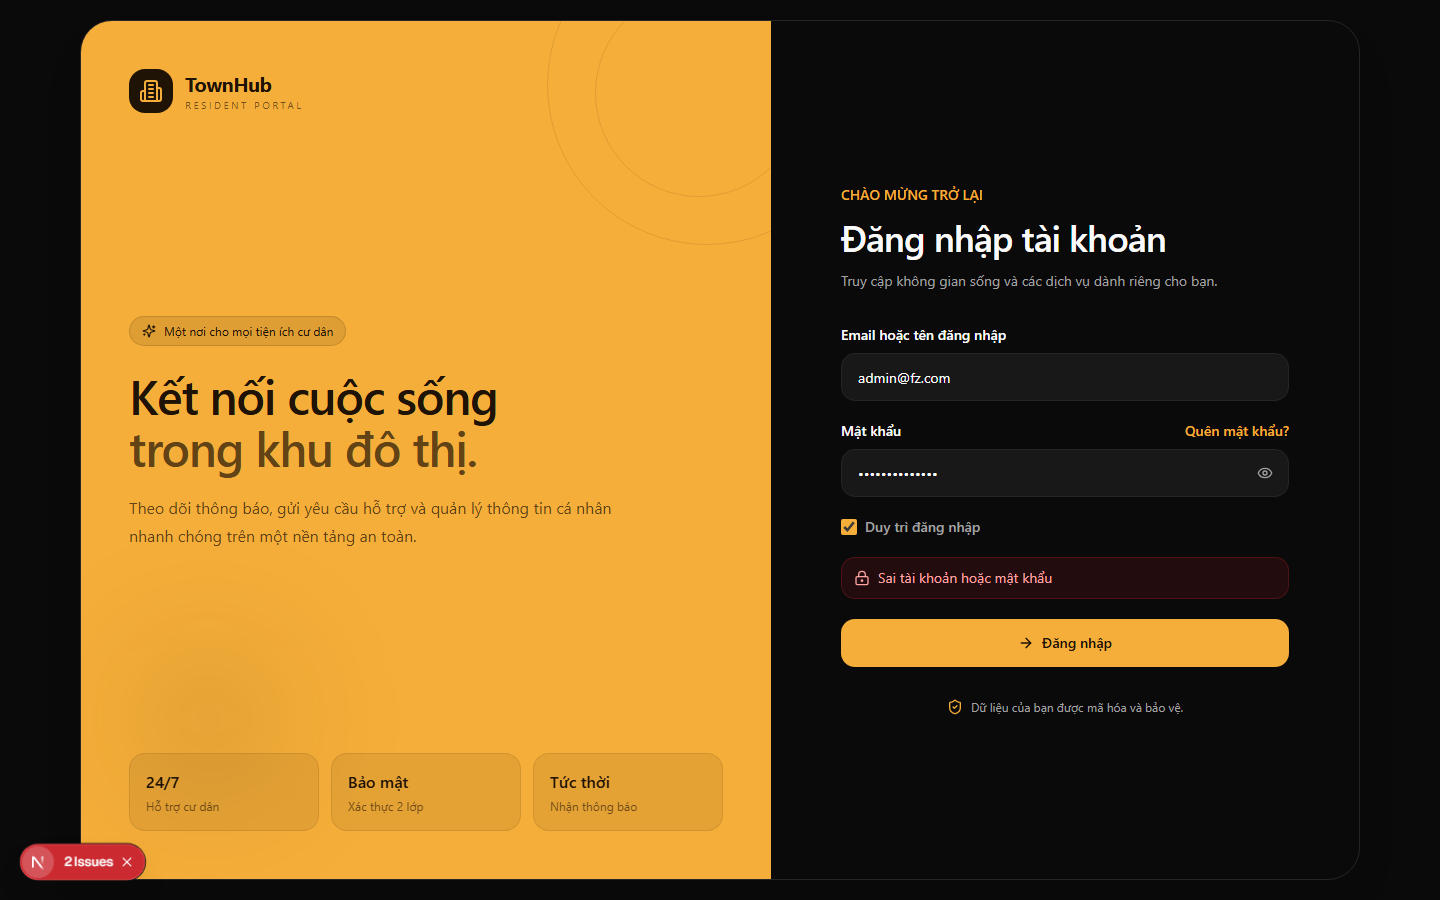
\includegraphics[width=\linewidth,height=0.44\textheight,keepaspectratio]{images/tc_auth_03_wrong_password.png}
\caption*{\small Hình PL.6. Ca side: đăng nhập sai mật khẩu bị báo lỗi.}
\end{figure}

\clearpage
\textbf{Ảnh minh hoạ 2 — Các màn hình nghiệp vụ được kiểm thử.}

\begin{figure}[H]\centering
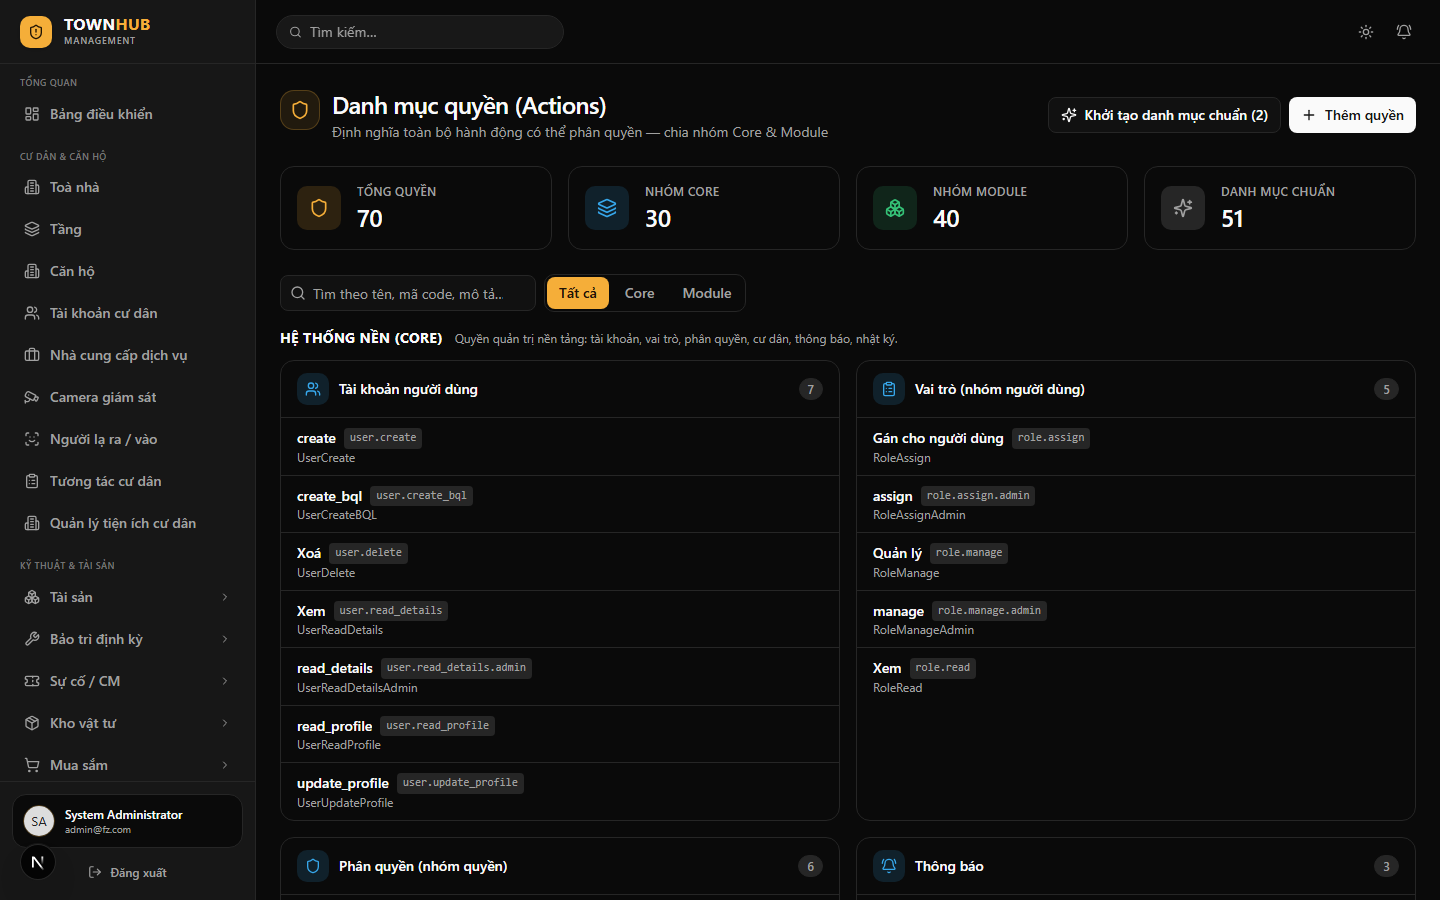
\includegraphics[width=\linewidth,height=0.44\textheight,keepaspectratio]{images/tc_auth_22_permissions.png}
\caption*{\small Hình PL.7. Danh mục quyền \& phân quyền (RBAC).}
\end{figure}
\begin{figure}[H]\centering
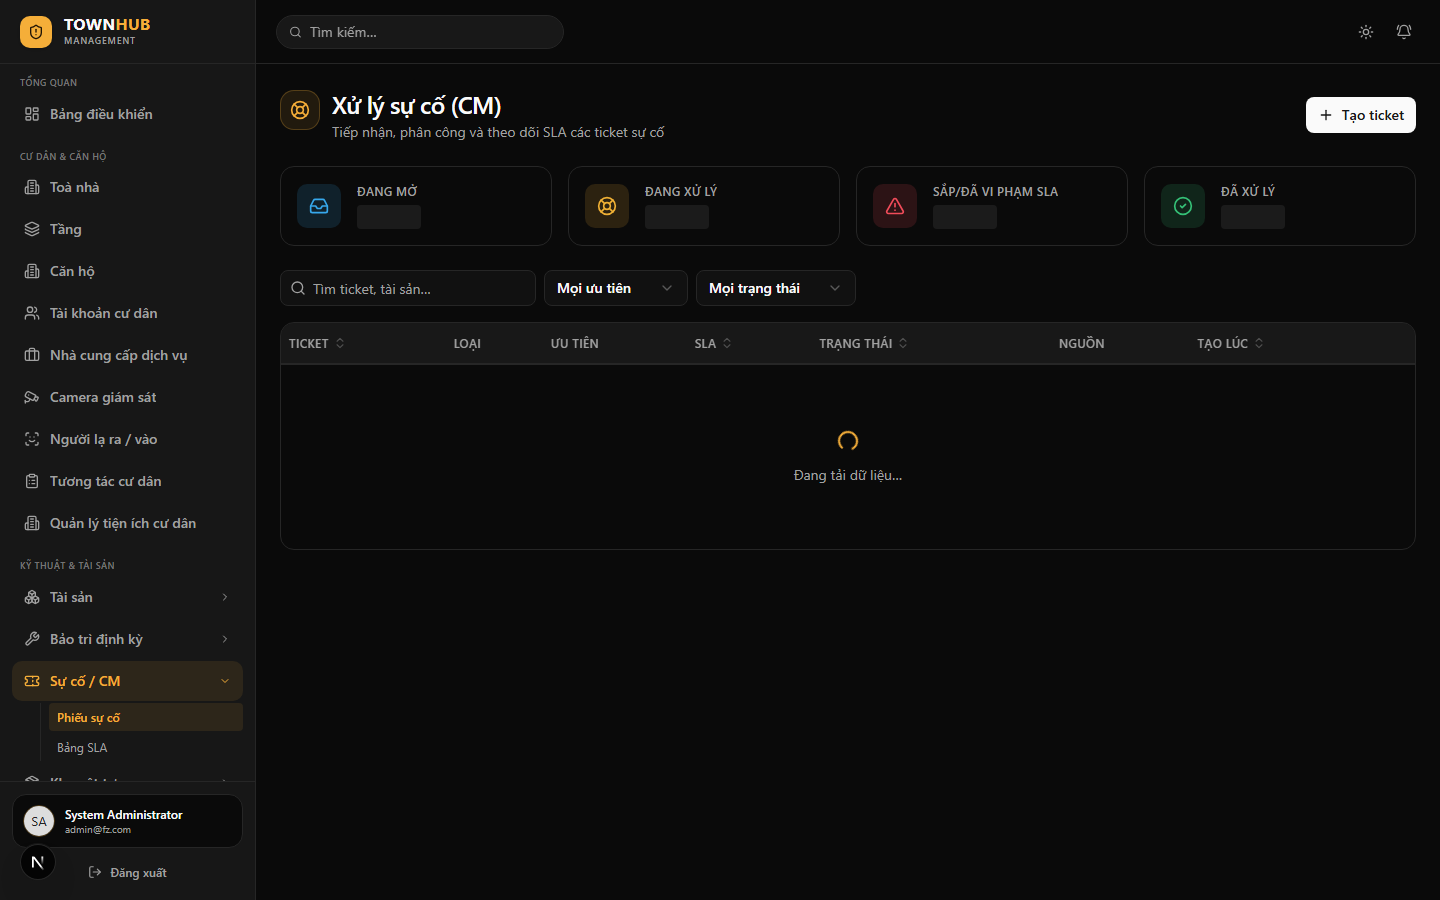
\includegraphics[width=\linewidth,height=0.44\textheight,keepaspectratio]{images/tc_ui_tickets.png}
\caption*{\small Hình PL.8. Danh sách ticket sự cố.}
\end{figure}
\begin{figure}[H]\centering
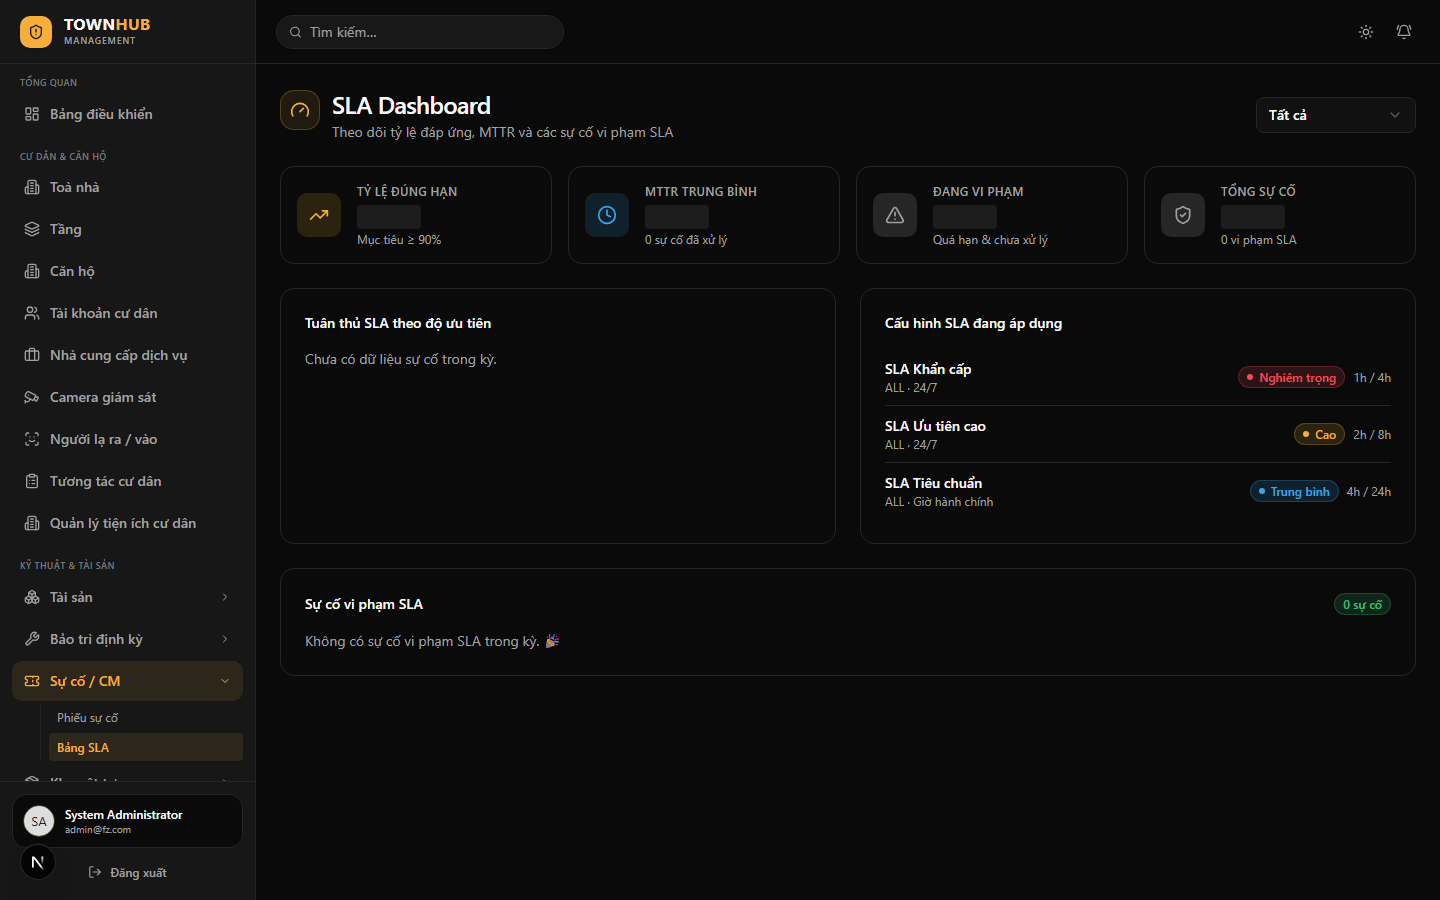
\includegraphics[width=\linewidth,height=0.44\textheight,keepaspectratio]{images/tc_ui_sla_dashboard.png}
\caption*{\small Hình PL.9. Bảng theo dõi SLA.}
\end{figure}
\clearpage
\begin{figure}[H]\centering
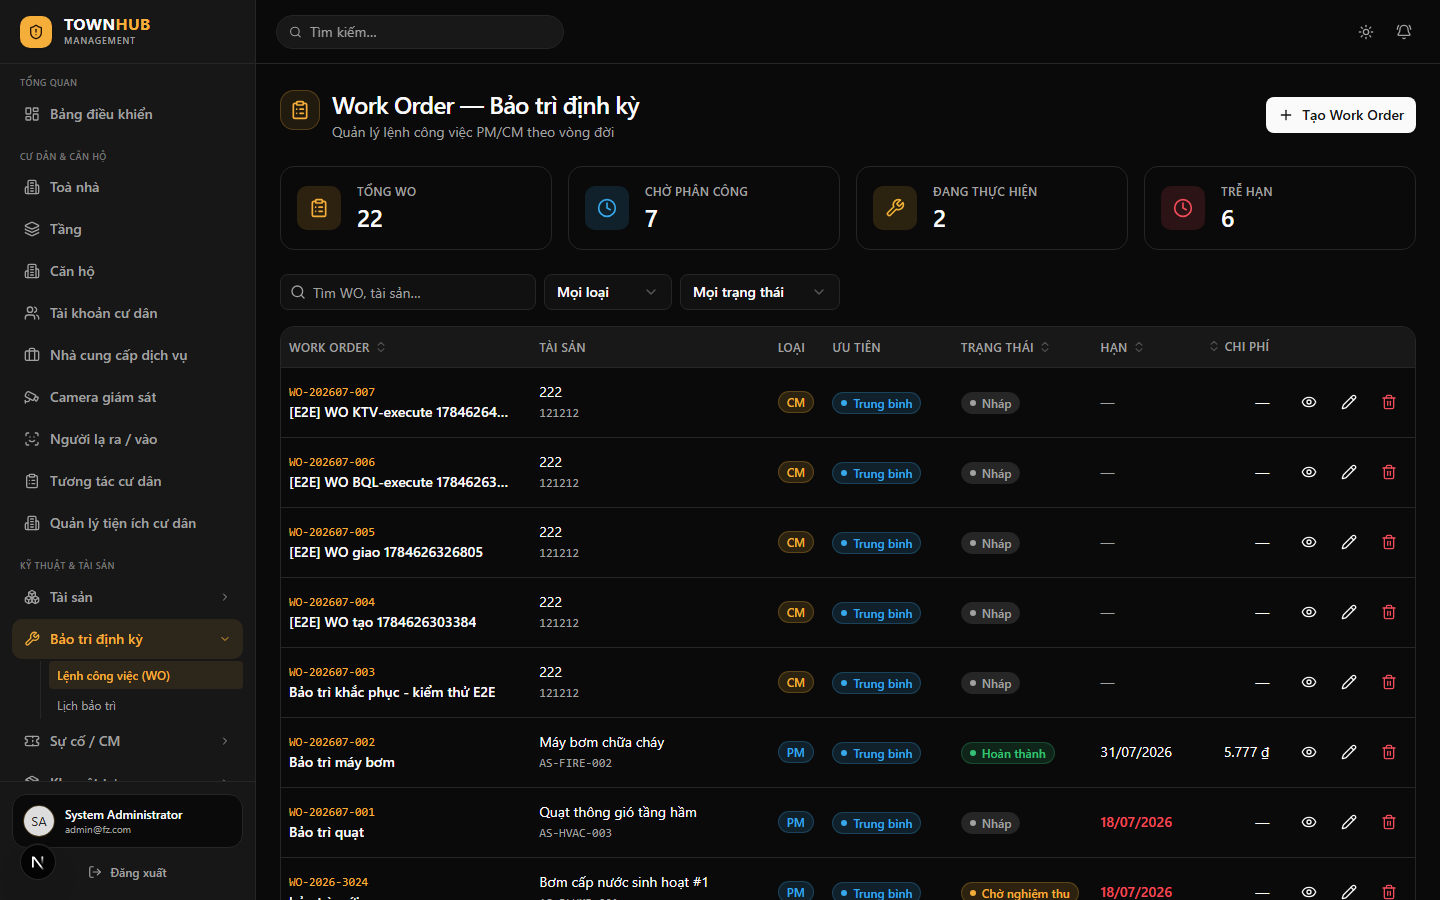
\includegraphics[width=\linewidth,height=0.44\textheight,keepaspectratio]{images/tc_ui_work_orders.png}
\caption*{\small Hình PL.10. Danh sách lệnh công việc (Work Order).}
\end{figure}
\begin{figure}[H]\centering
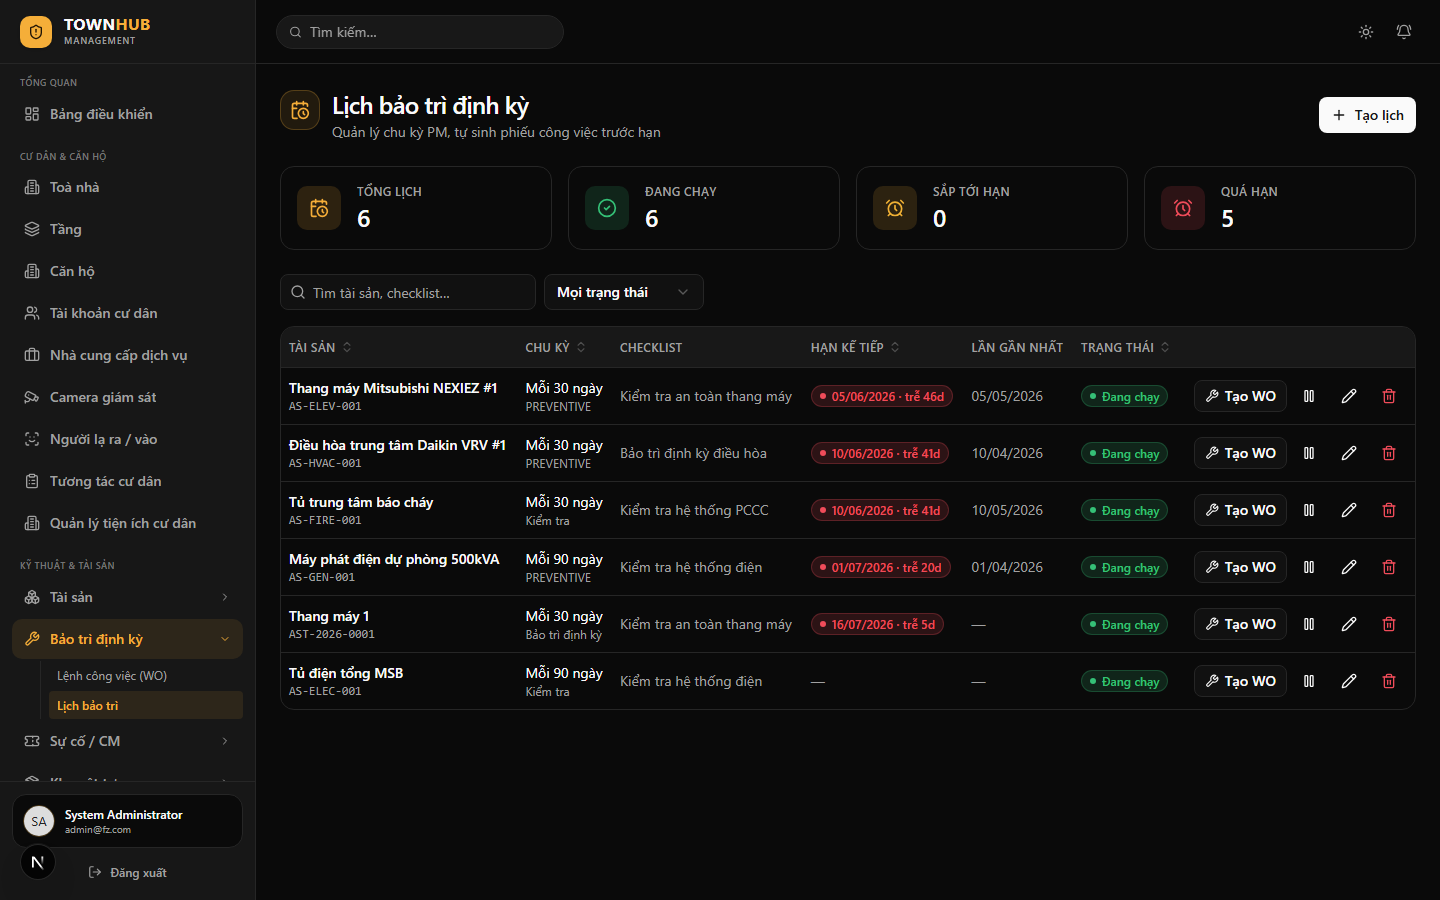
\includegraphics[width=\linewidth,height=0.44\textheight,keepaspectratio]{images/tc_ui_pm_schedules.png}
\caption*{\small Hình PL.11. Lịch bảo trì định kỳ.}
\end{figure}
\begin{figure}[H]\centering
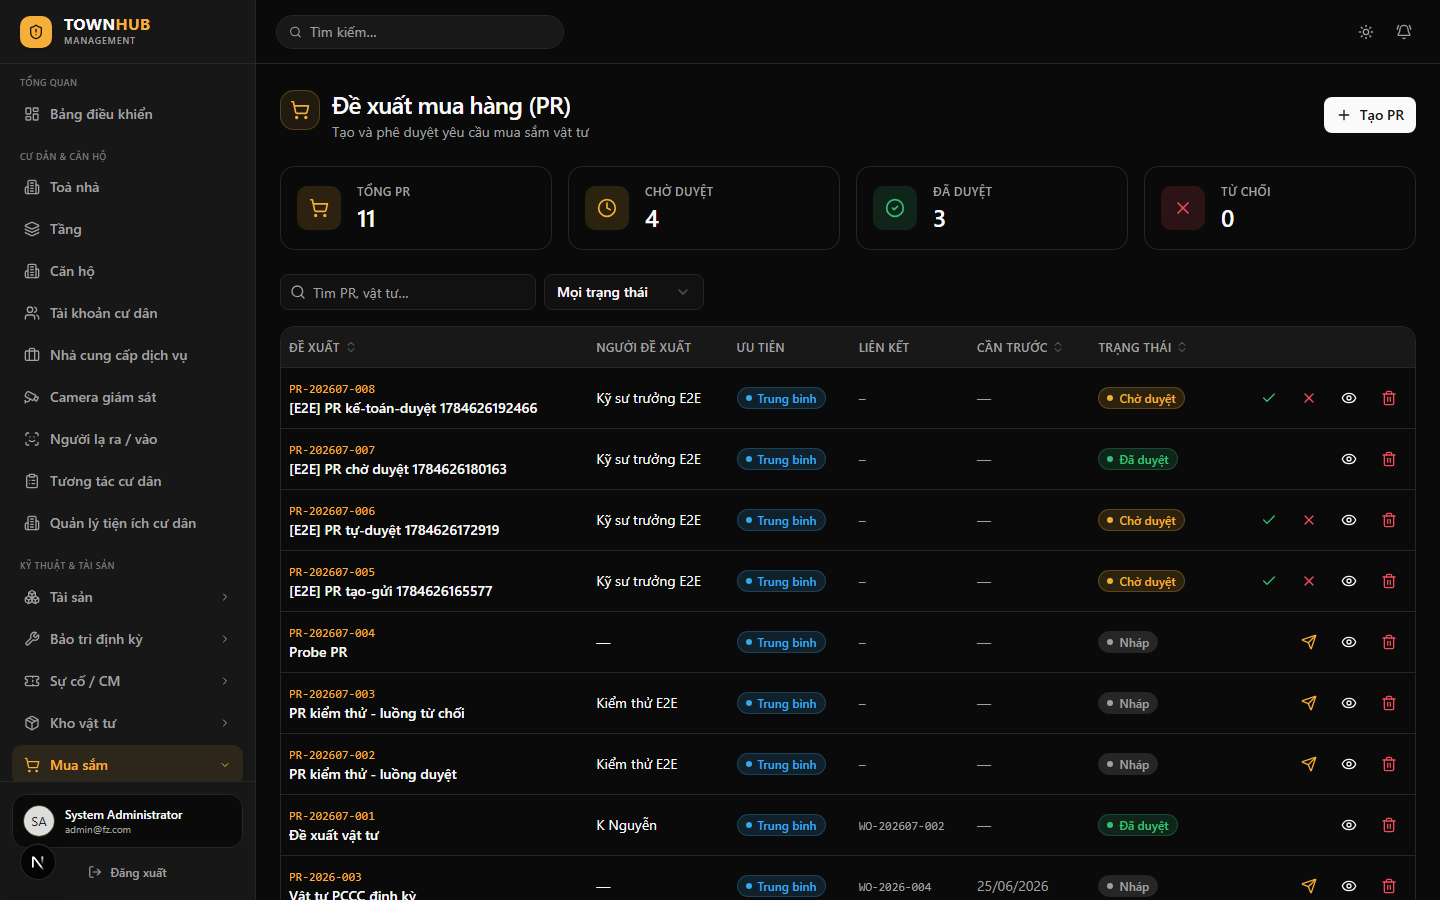
\includegraphics[width=\linewidth,height=0.44\textheight,keepaspectratio]{images/tc_ui_proc_requests.png}
\caption*{\small Hình PL.12. Phiếu yêu cầu mua sắm (PR).}
\end{figure}
\clearpage
\begin{figure}[H]\centering
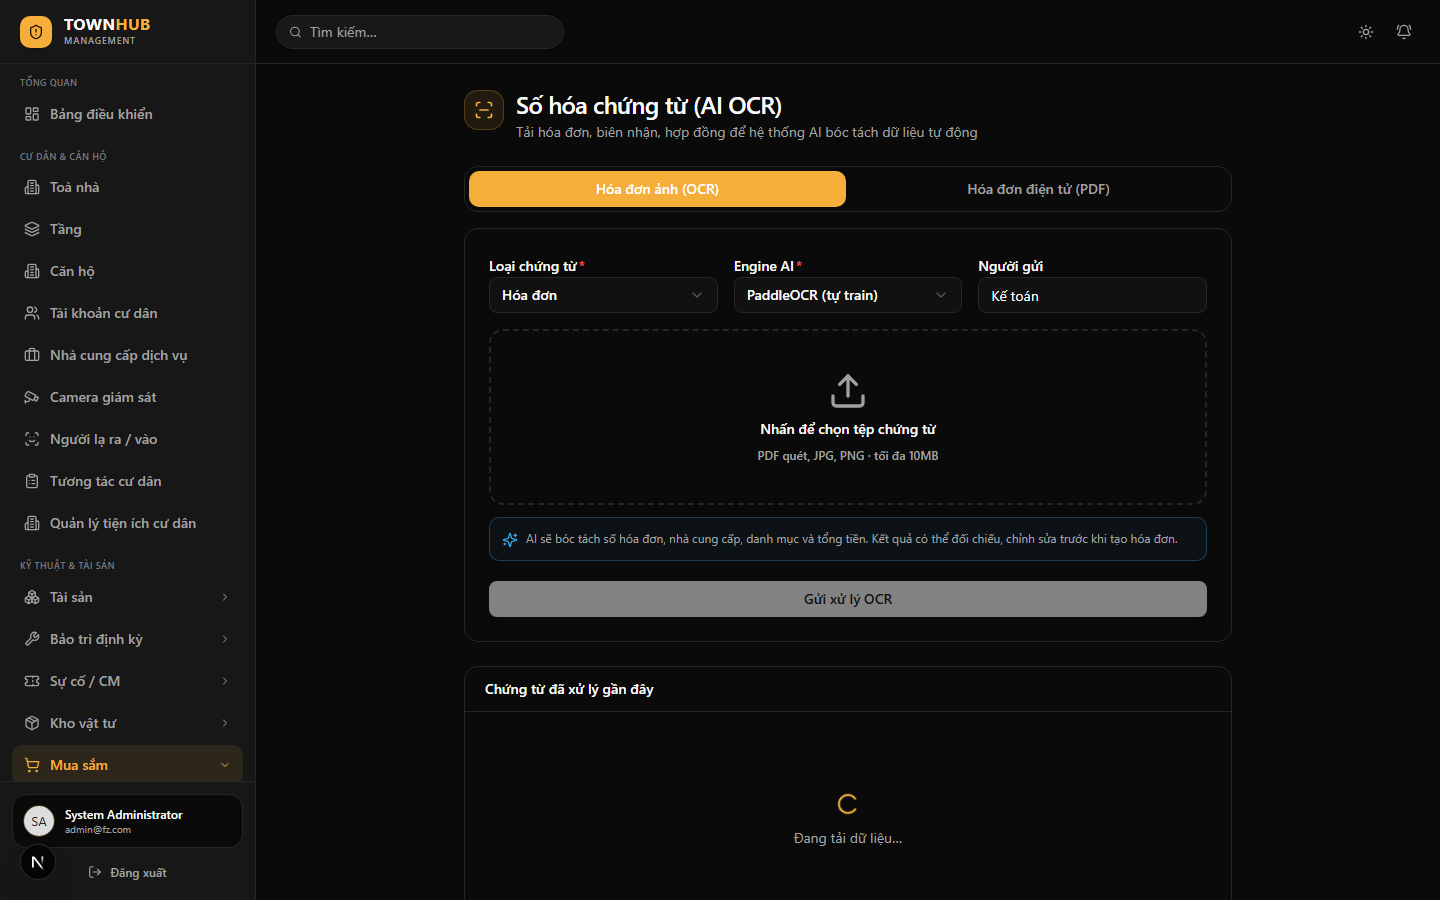
\includegraphics[width=\linewidth,height=0.44\textheight,keepaspectratio]{images/tc_ui_proc_ocr_new.png}
\caption*{\small Hình PL.13. Màn hình tải hoá đơn cho OCR.}
\end{figure}
\begin{figure}[H]\centering
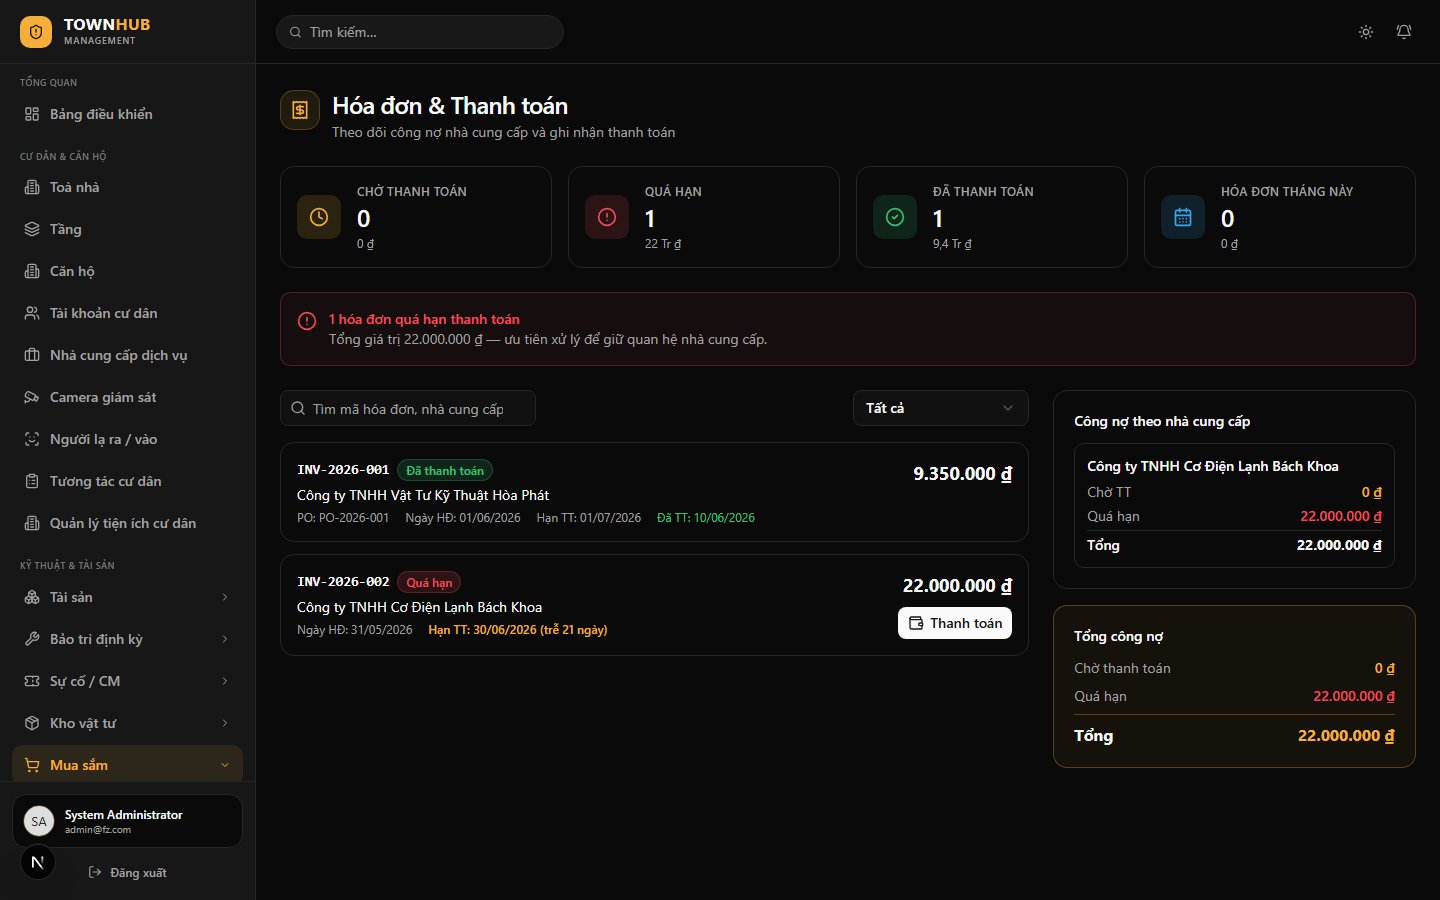
\includegraphics[width=\linewidth,height=0.44\textheight,keepaspectratio]{images/tc_ui_proc_invoices.png}
\caption*{\small Hình PL.14. Danh sách hoá đơn.}
\end{figure}
\begin{figure}[H]\centering
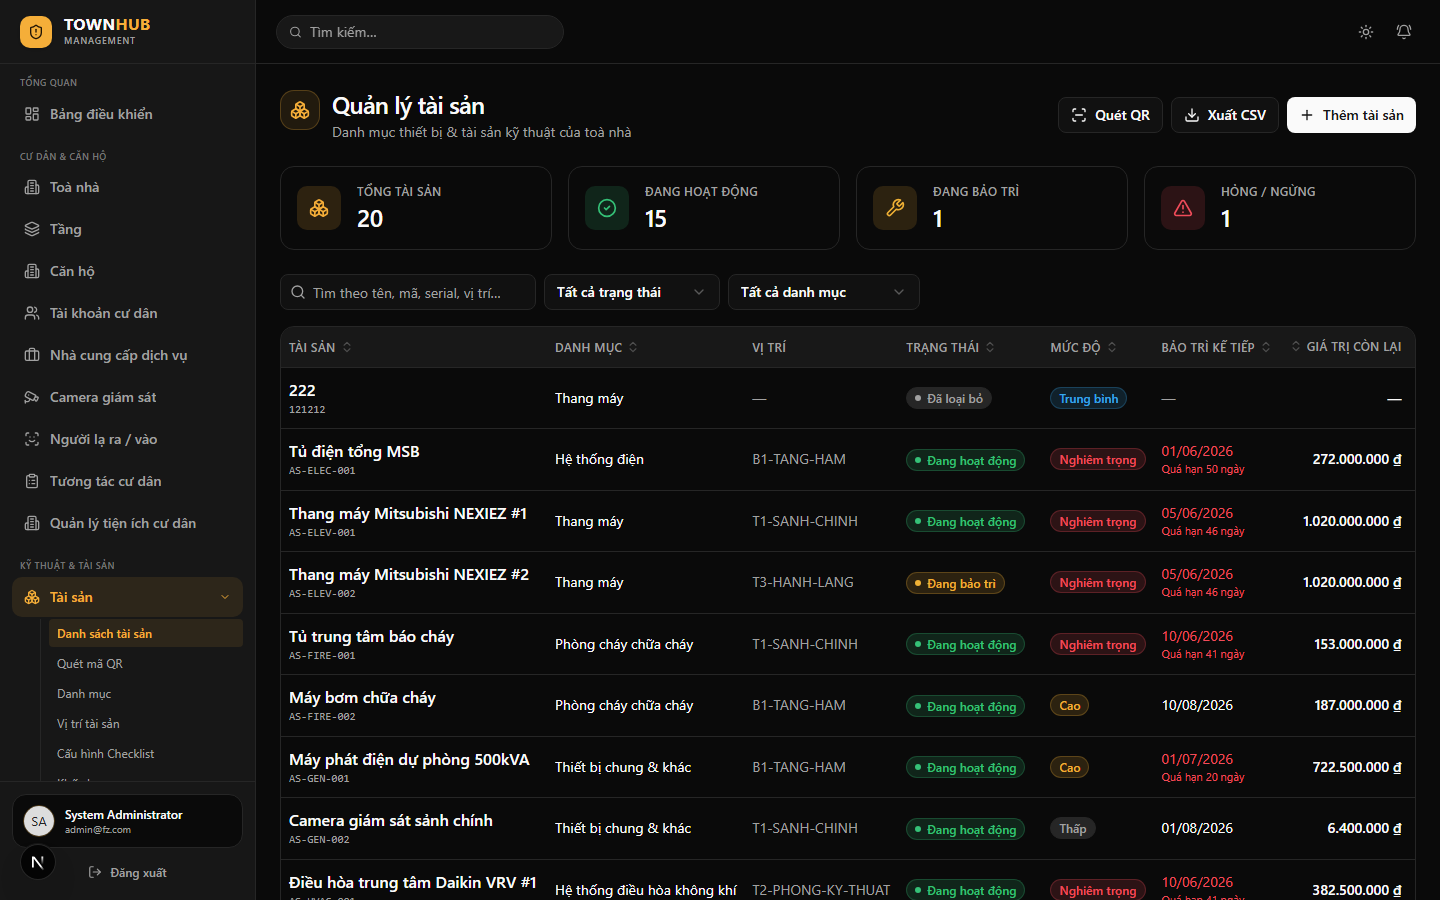
\includegraphics[width=\linewidth,height=0.44\textheight,keepaspectratio]{images/tc_ui_assets_list.png}
\caption*{\small Hình PL.15. Danh sách tài sản.}
\end{figure}
\clearpage
\begin{figure}[H]\centering
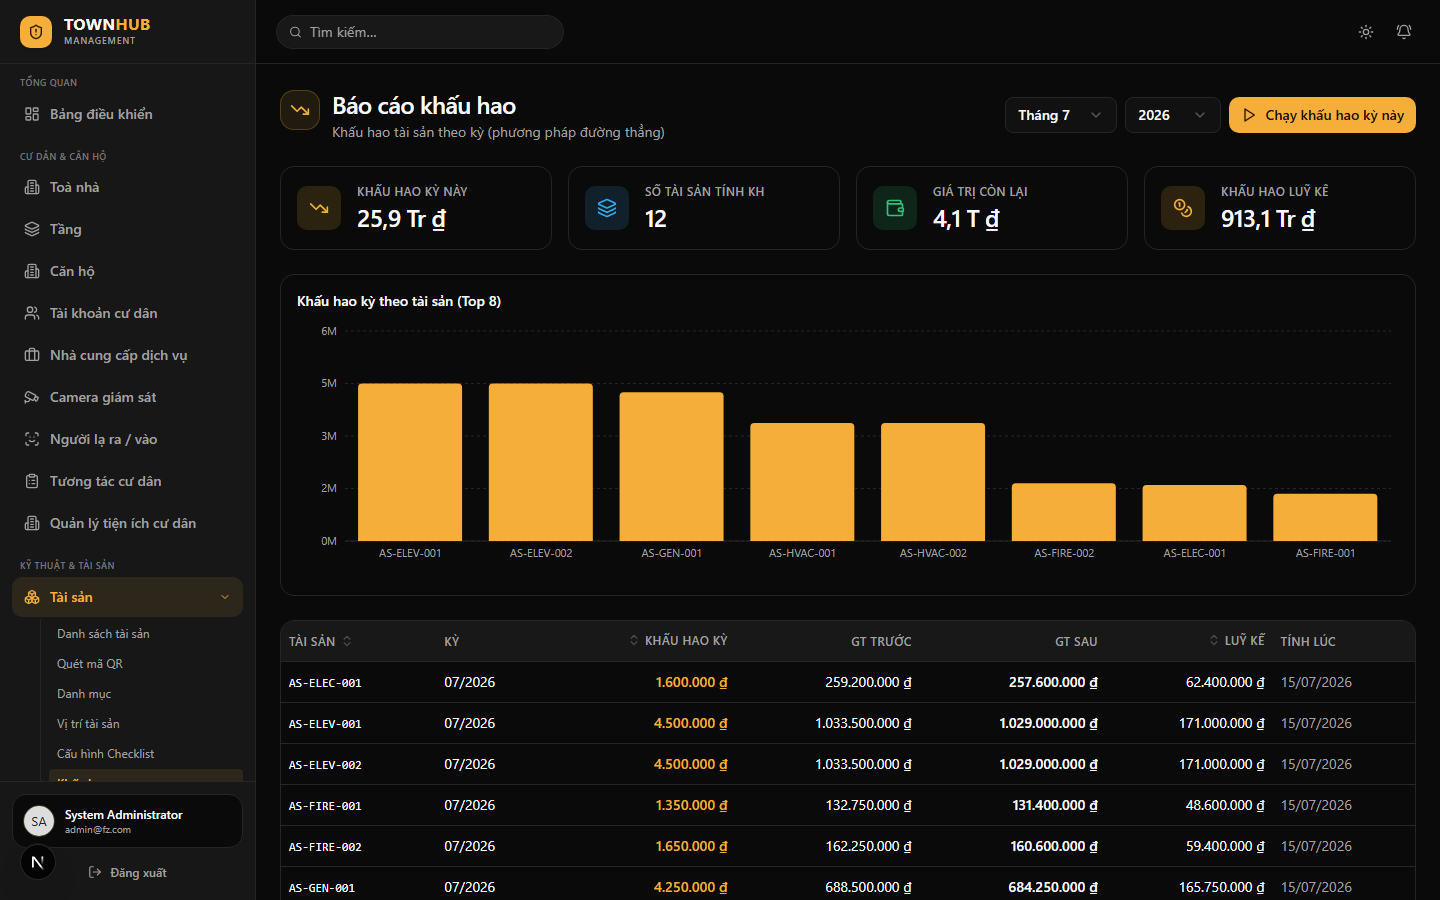
\includegraphics[width=\linewidth,height=0.44\textheight,keepaspectratio]{images/tc_ui_assets_depreciation.png}
\caption*{\small Hình PL.16. Khấu hao tài sản.}
\end{figure}
\begin{figure}[H]\centering
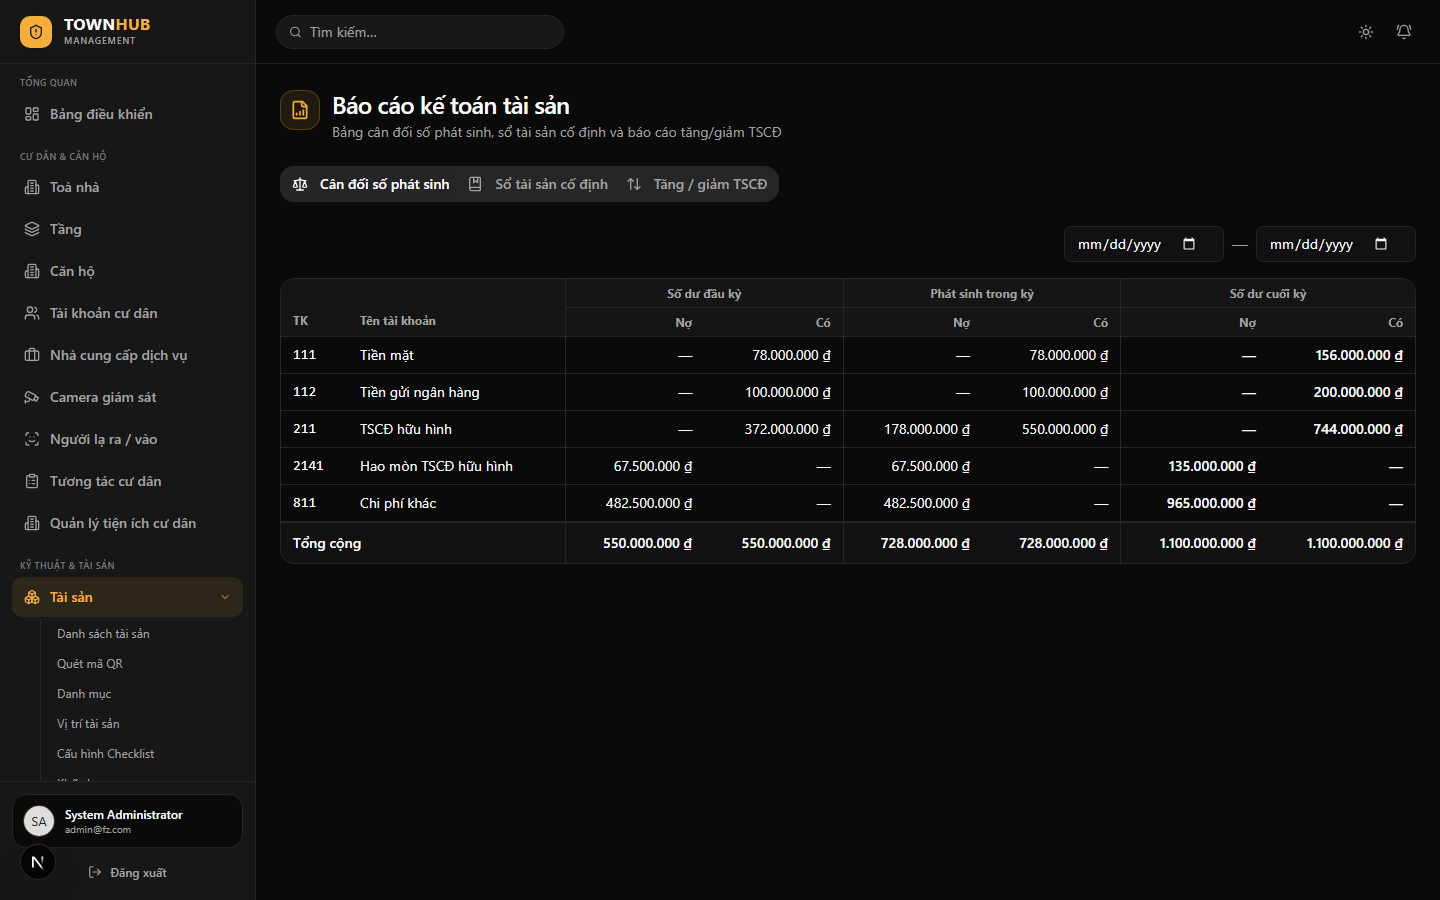
\includegraphics[width=\linewidth,height=0.44\textheight,keepaspectratio]{images/tc_ui_assets_reports.png}
\caption*{\small Hình PL.17. Báo cáo tài sản (kế toán).}
\end{figure}
